\documentclass{article}

\usepackage{color}
\usepackage{graphicx}
\usepackage{tabularx}


\usepackage{geometry}
 \geometry{
 top=25mm,
 bottom=25mm,
 }


\title{Document de presentation}
\author{Justal Kevin}
\date{26/09/2015}
\renewcommand{\contentsname}{Table des matieres} 
 
\newcommand\invisiblesection[1]{%
  \refstepcounter{section}%
  \addcontentsline{toc}{section}{\protect\numberline{\thesection}#1}%
  \sectionmark{#1}} 
 
\begin{document}

\begin{center}
\textbf{\Huge{LES ANIMAUX}}
\line(1,0){300}\\
NOTICE DU JEU\\
\vspace{3cm}
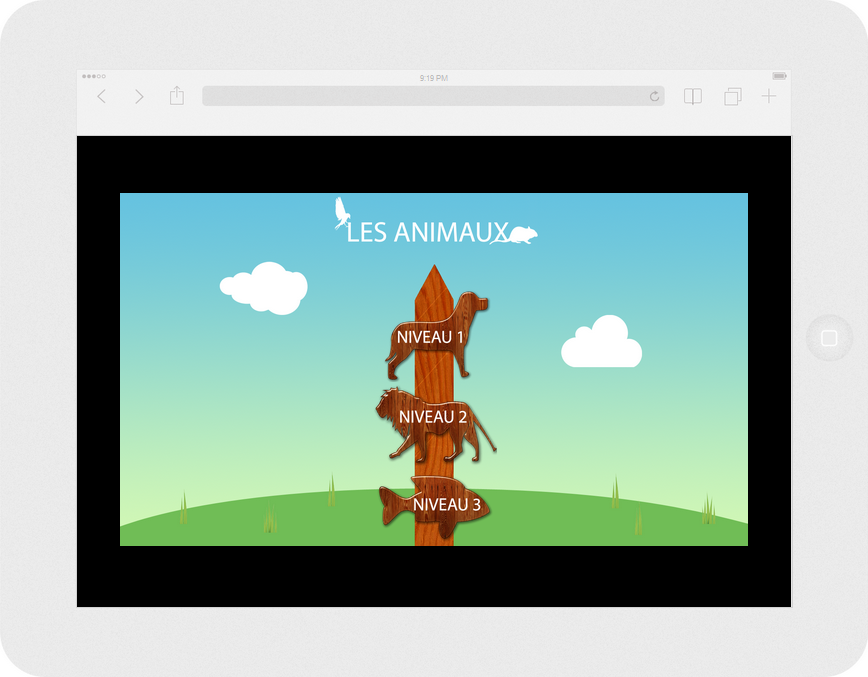
\includegraphics[width=0.8\textwidth]{tablette}\\
\vspace{3cm}
\textbf{Pr\'eambule}
\end{center}

\hspace*{0.6cm}Les jeux sont un bon moyen d'am\'eliorer les comp\'etence logico-math\'ematique et corporelle kinesth\'esique d'une personne. Mais ces effets sont d\'ecupl\'es sur des enfants. Pouss\'e par leur curiosit\'e et leur d\'esirs d'accomplissements, ils feront souvent tout ce qui est en leur pouvoir pour arriver \`a la fin d'un jeu. Ces sentiments, si bien mani\'es, peuvent permettre d'enseigner facilement \'enormement de choses aux enfants qu'ils soit handicap\'es ou non.
\vspace{0.5cm}\\
\hspace*{0.6cm}Notre jeu met le joueur devant un problème d'association logique entre plusieurs images. En d\'ebut de partie, cinq images sont donn\'es au joueur et 3 images en jaune sont quand \`a elles pos\'es devant lui. Le joueur doit alors chercher le lien entre les images qu'il a et celle en jaune.

\newpage
\tableofcontents

\newpage
\section{Pr\'erequis}
1. Un logiciel de d\'ecompression
\begin{itemize}
  \item Winrar
  \item Winzip (Install\'e de base avec windows)
\end{itemize}
2. Un navigateur web 
\begin{itemize}
  \item Internet explorer (Version minimum 9)
  \item Google Chrome (Version minimum 44)
  \item Mozilla Firefox (Version minimum 40)
  \item Safari (Version minimum 5.1)
  \item Opera (Version minimum 12)
  \item iOS (Version minimum 6.1)
  \item Android (Version minimum 2.3)
\end{itemize}

\newpage
\section{Installation}
\subsection{D\'ecompression}
\hspace*{0.6cm}D\'ecompresser l'archive par un simple clique droit puis extraire ici comme le montre l'image ci-dessous :\\
(Une installation de winrar sera peut-\^etre n\'ecessaire)
\vspace{0.5cm}\\
\fbox{
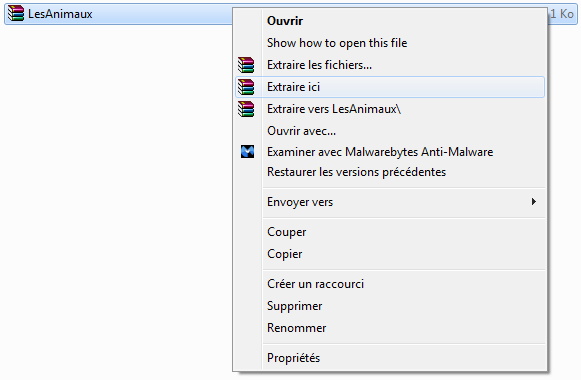
\includegraphics[width=1.0\textwidth]{winrar}\\
}
\subsection{Lancement}
Cliquer ensuite sur le dossier apparu et cliquer sur le fichier nomm\'e "index" ou "index.html" :
\vspace{0.5cm}\\
\fbox{

\includegraphics[width=1.0\textwidth]{index}\\
}
\subsection{Plein \'Ecran}
Il est possible de mettre le jeu en plein \'ecran en cliquant sur F11 une fois le jeu arriv\'e sur l'\'ecran d'accueil. 

\newpage
\section{Gameplay}

Le jeu est d\'ecompos\'e en deux parties. En haut (zone1 en rouge), vous trouverez les animaux que vous pouvez d\'eplacer et en bas (zone 2 en violet) les zones o\`u vous pouvez les d\'eplacer.
\vspace{0.5cm}\\
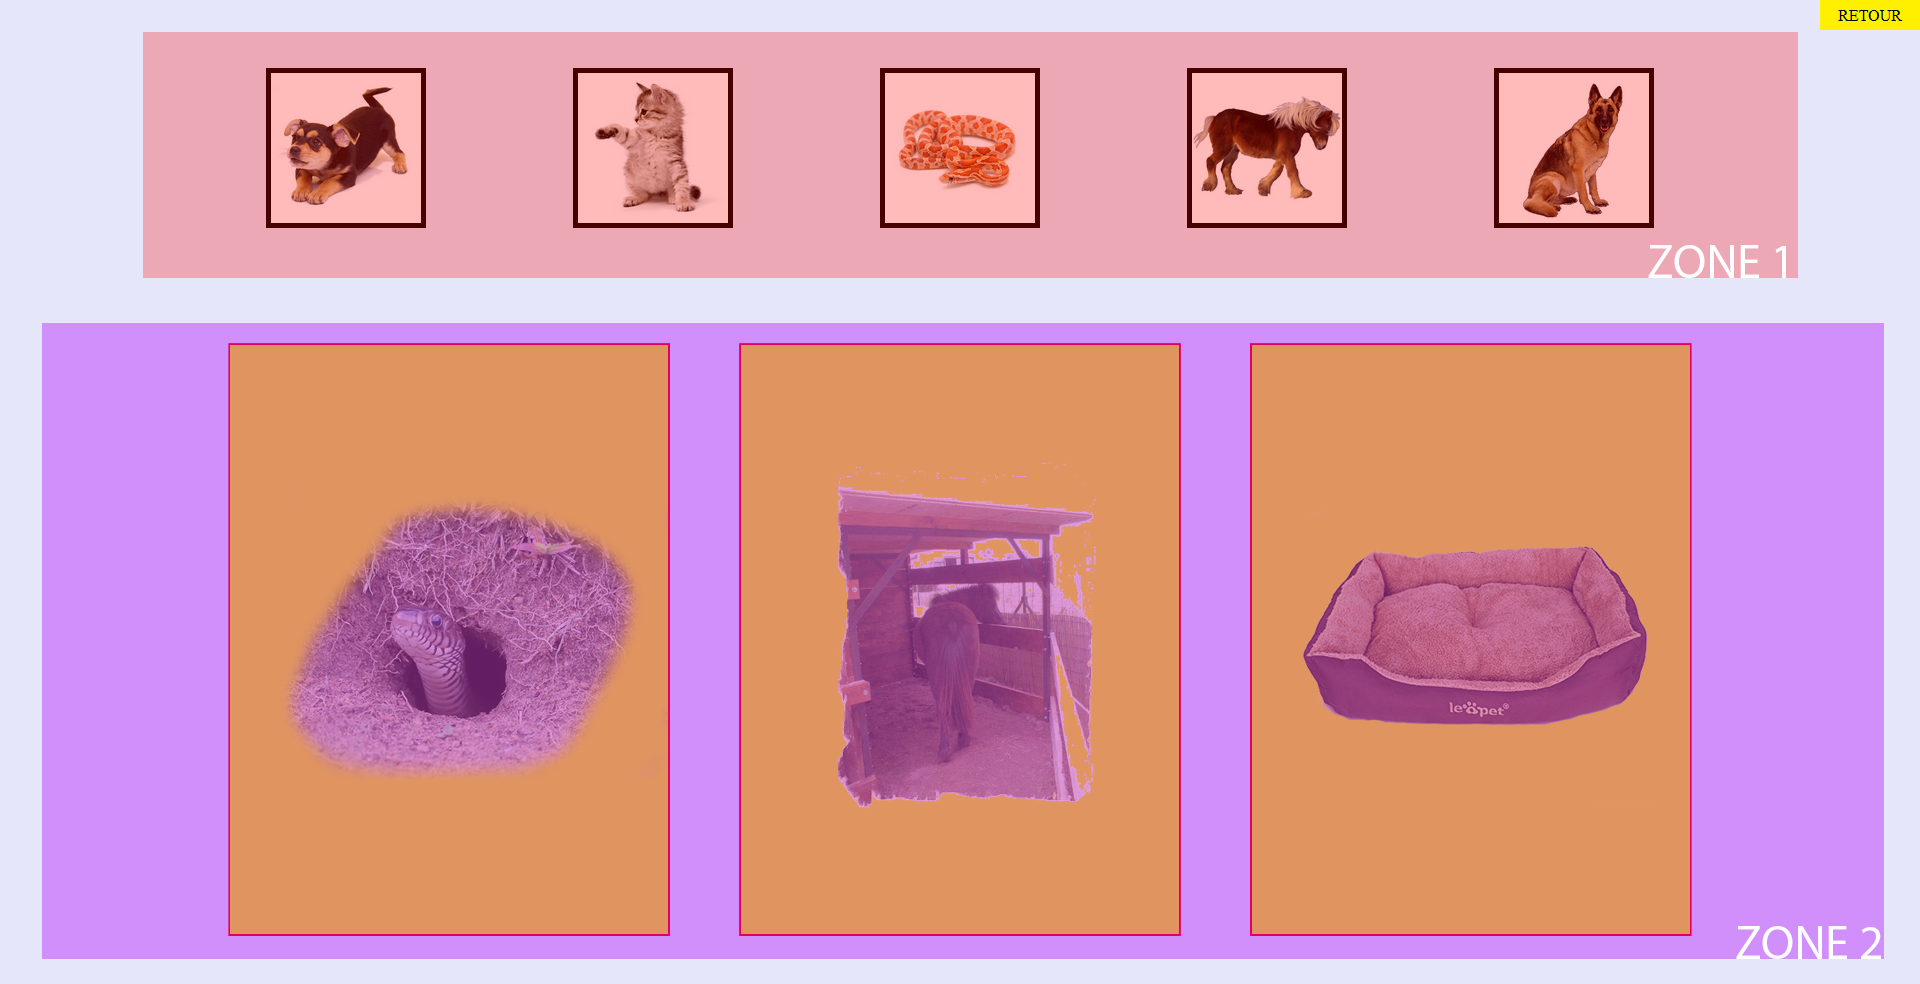
\includegraphics[width=1.0\textwidth]{zone}
\vspace{0.5cm}\\
Le but du jeu est d\'eplacer les animaux de la zone 1 vers la zone 2 en suivant une certaine logique. Reprenons notre exemple pr\'ec\'edent et notons les animaux de la zone 1.\\
\vspace{0.5cm}\\
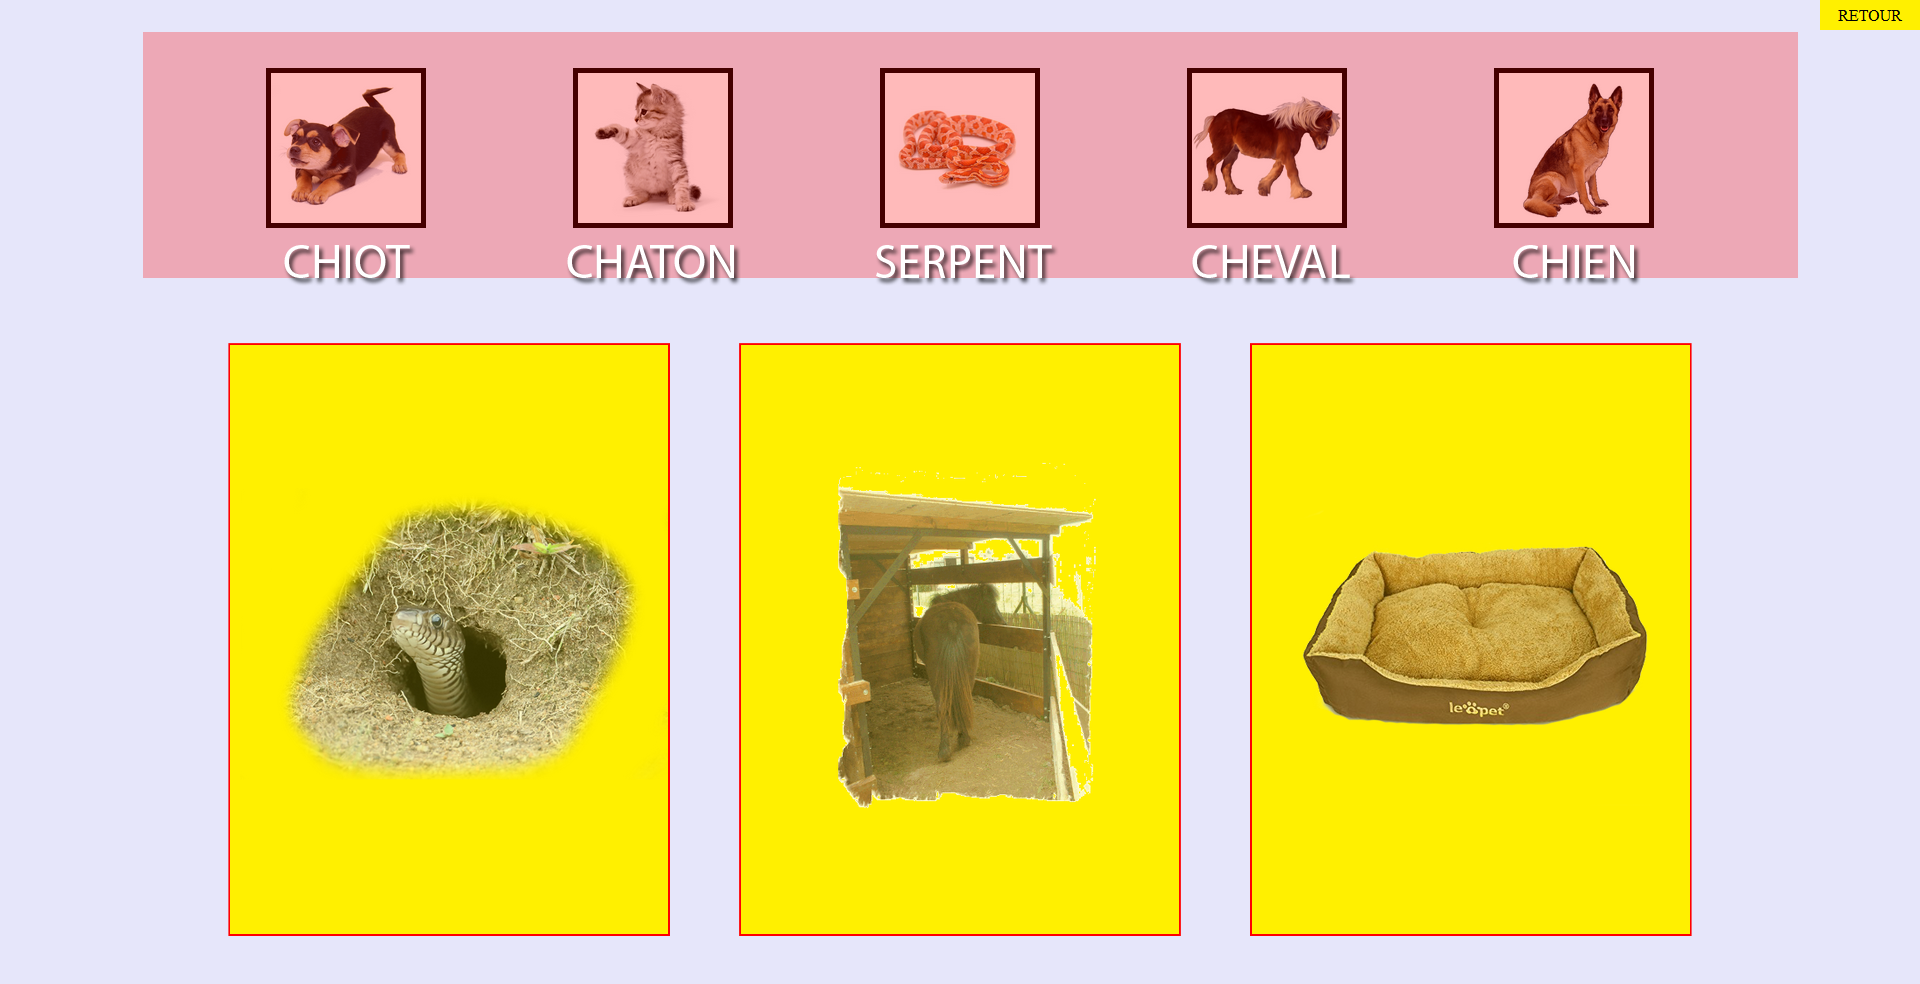
\includegraphics[width=1.0\textwidth]{zone1}
\vspace{0.5cm}\\
Prenons par exemple le cheval, nous allons cliquer dessus et maintenir notre clique tout en d\'epla\c{c}ant la souris.
\vspace{0.5cm}\\
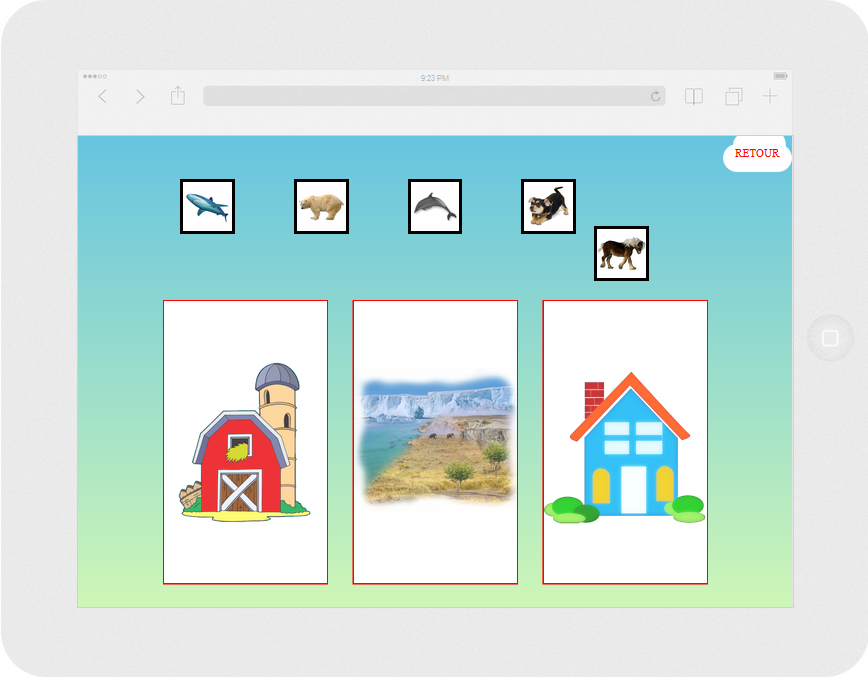
\includegraphics[width=1.0\textwidth]{zone2}
\vspace{0.5cm}\\
Si nous rel\^achons notre clique, l'image du cheval retournera \'a sa place automatiquement. Maintenant, regardons avec attention la zone 2 et d\'ecrivons l\`a aussi les images. 
\vspace{0.5cm}\\
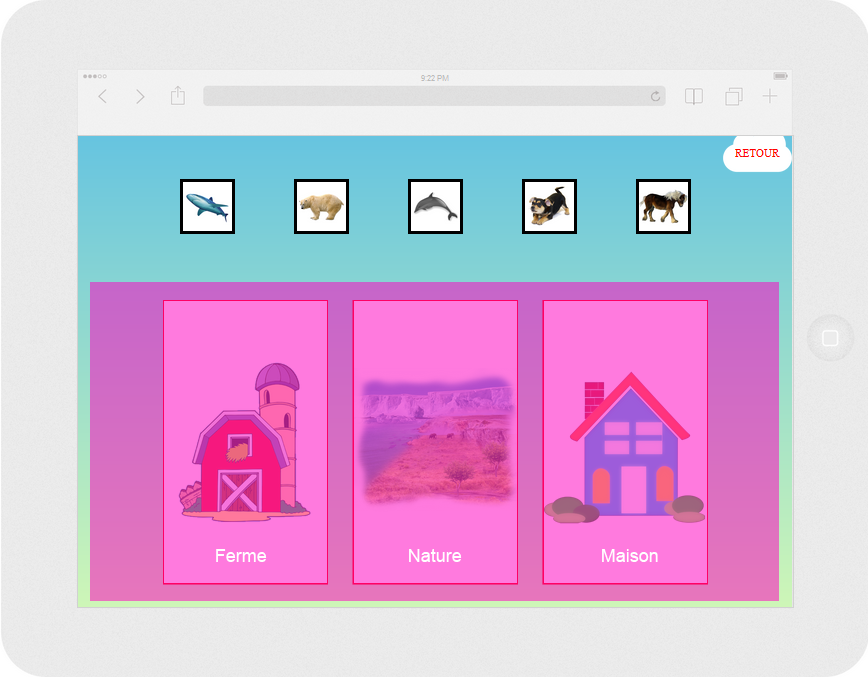
\includegraphics[width=1.0\textwidth]{zone3}
\vspace{0.5cm}\\
Reprenons maintenant notre cheval et d\'epla\c{c}ont le dans la zone qui lui correspond (l'écurie). L'image se fixera alors \`a la zone et vous ne pourrez plus y toucher. Vous avez la bonne r\'eponse !
\vspace{0.5cm}\\
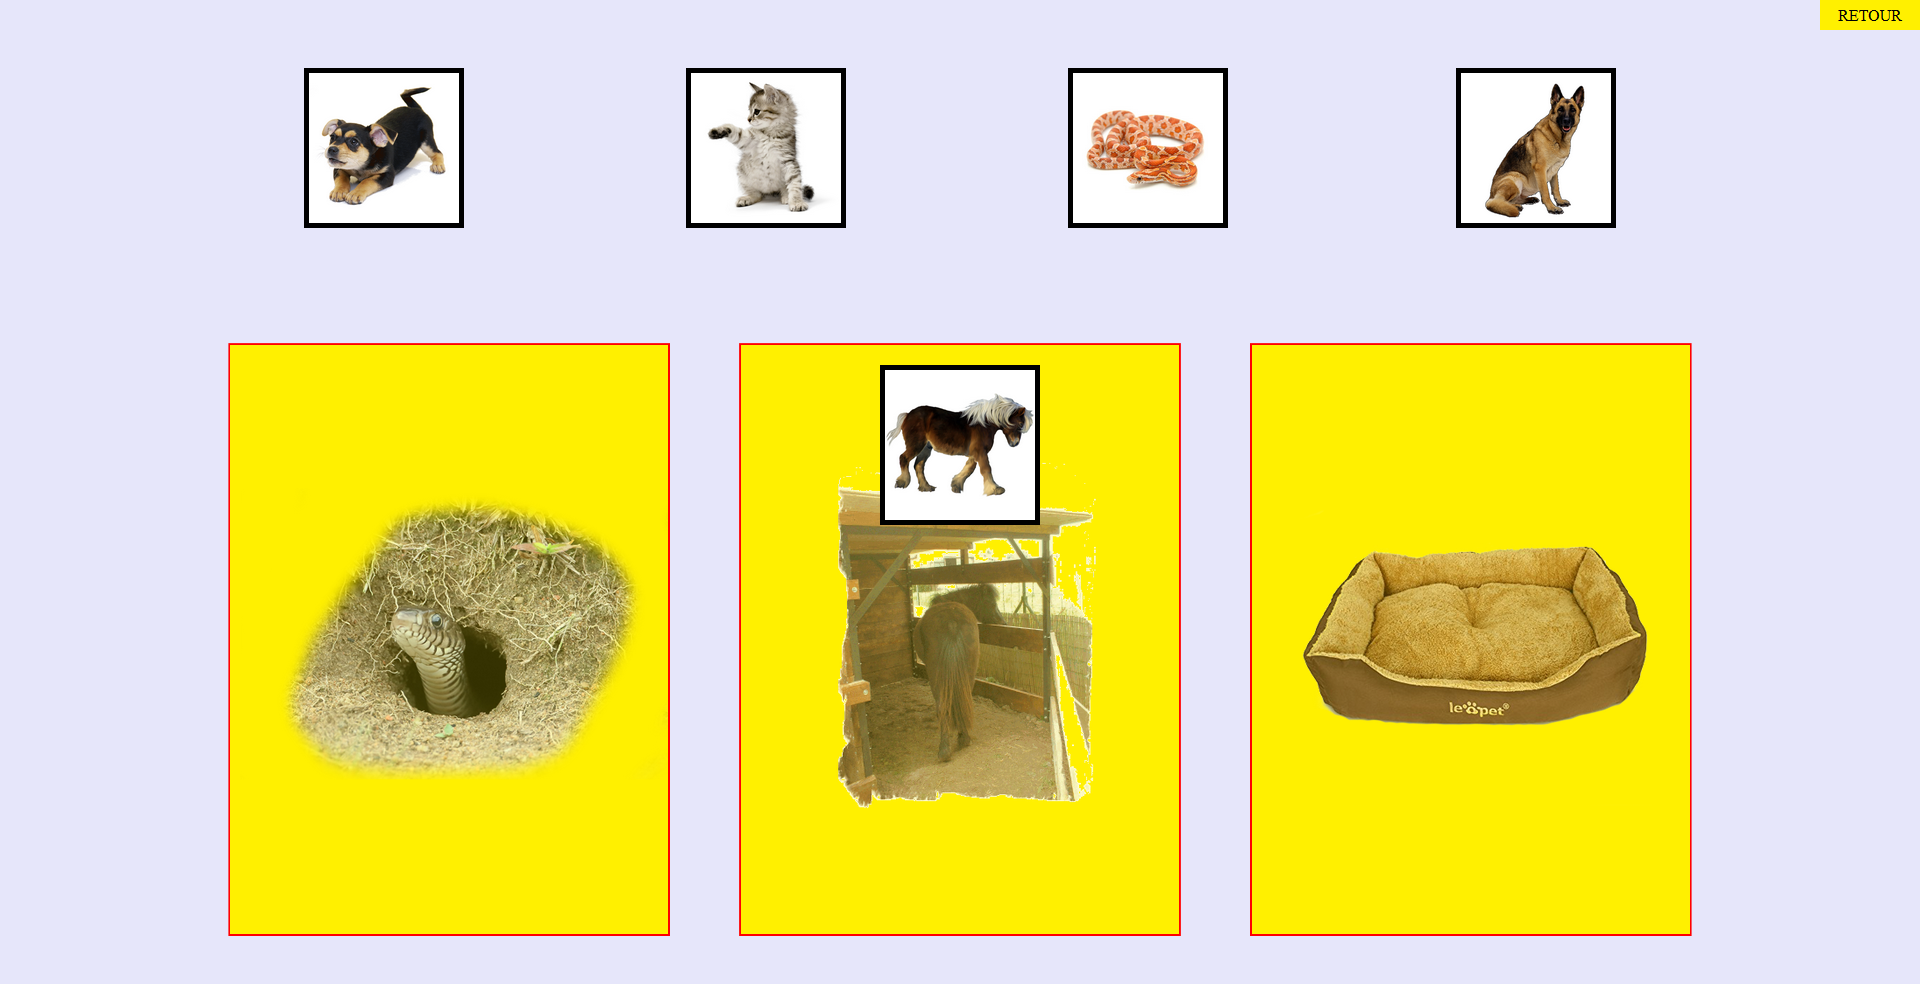
\includegraphics[width=1.0\textwidth]{zone4}
\vspace{0.5cm}\\
Maintenant effectuons cette m\^eme op\'eration pour chaque image restante dans la zone 1. Allez, encore un petit effort, nous y somme presque.
\vspace{0.5cm}\\
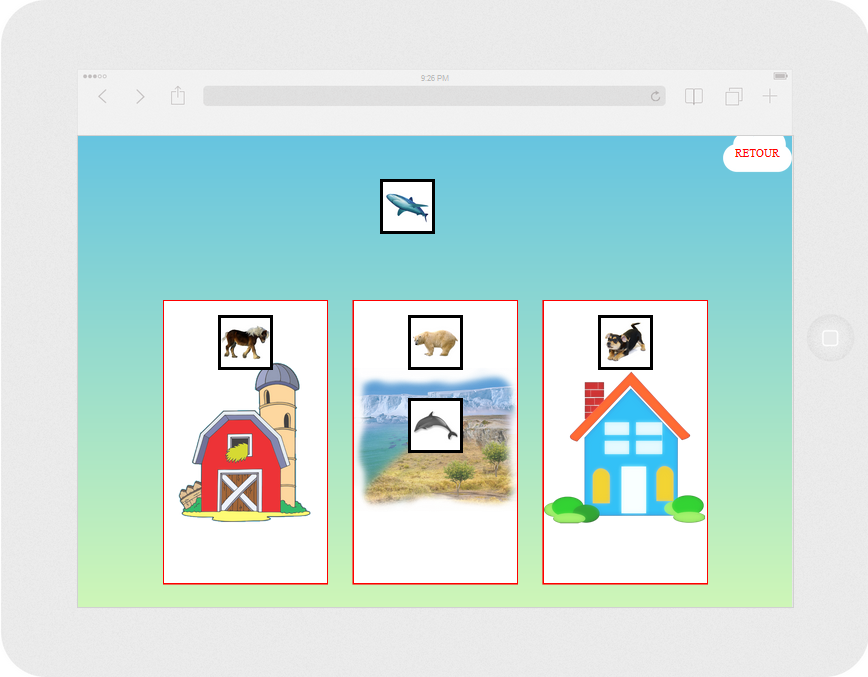
\includegraphics[width=1.0\textwidth]{zone5}
\vspace{0.5cm}\\
Si vous r\'epondez correctement en pla\c{c}ant l'integralit\'e des images, un message vous disant "Bravo" s'affiche alors pour vous f\'eliciter.
\vspace{0.5cm}\\
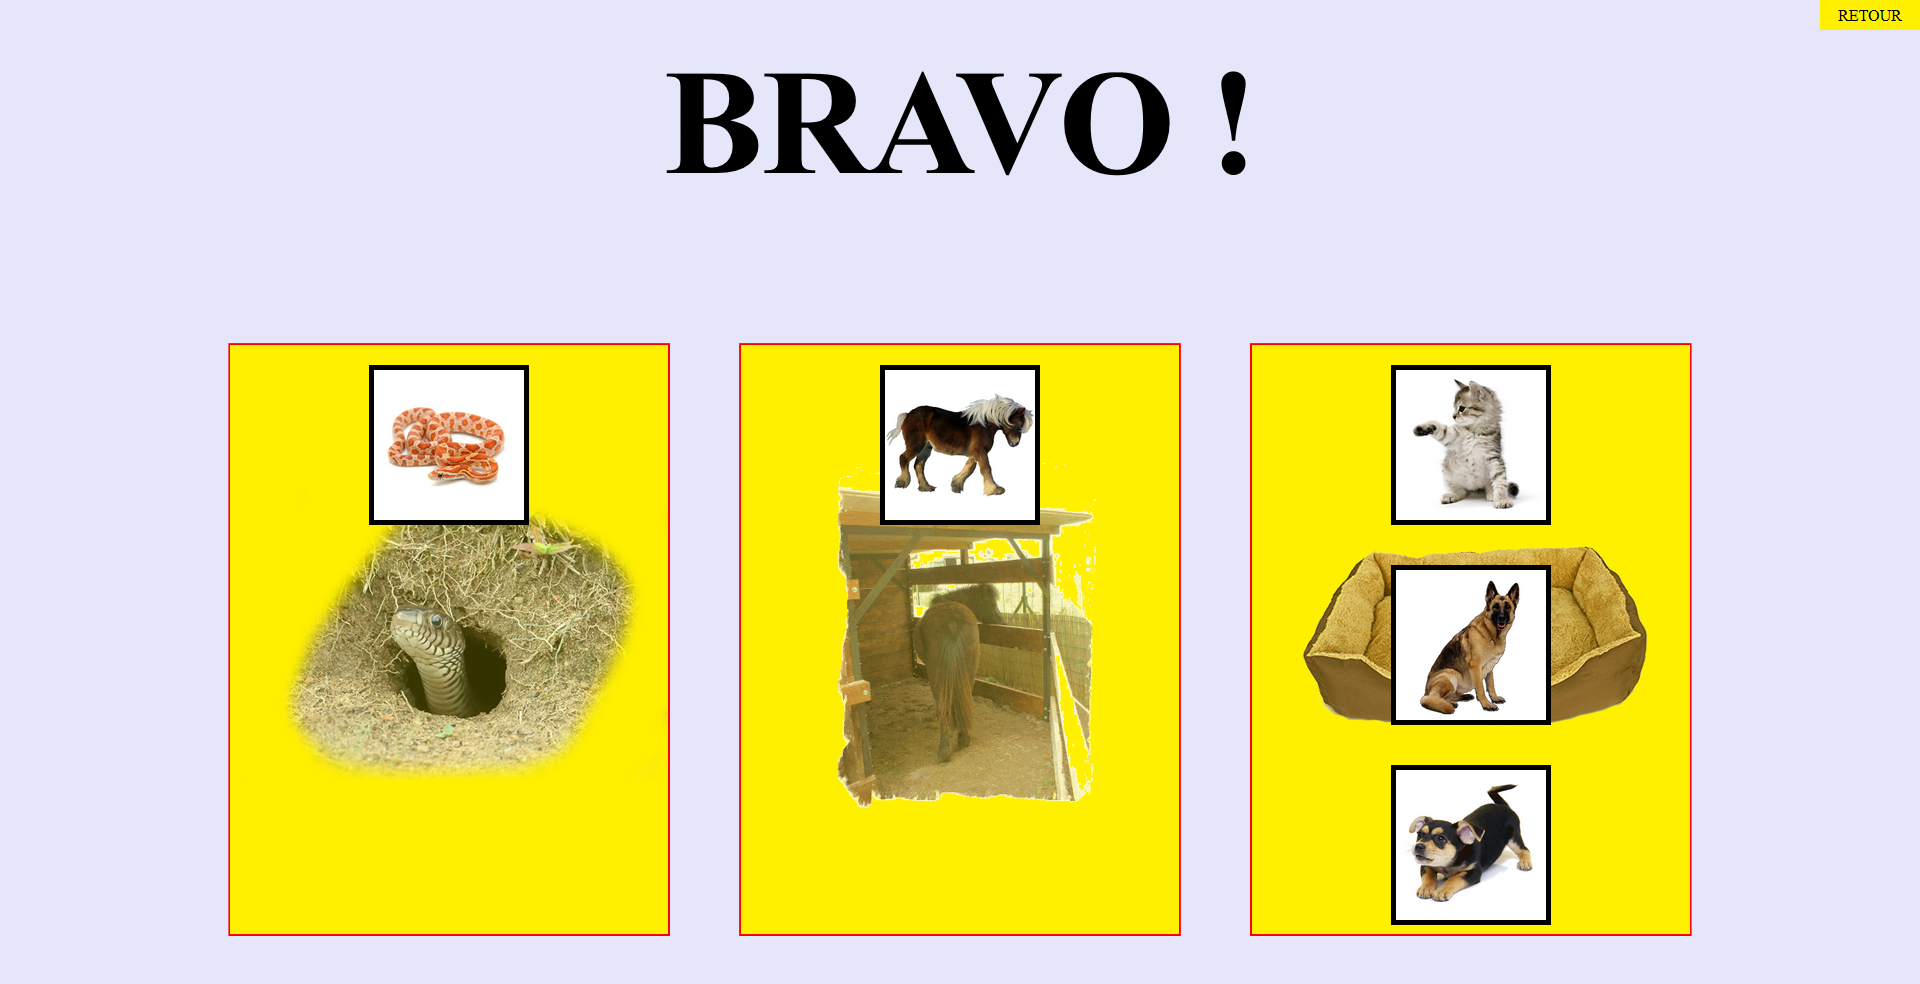
\includegraphics[width=1.0\textwidth]{zone6}
\vspace{0.5cm}\\
Puis une nouvelle partie commence avec de nouveaux \'el\'ement dans les deux zones.
\vspace{0.5cm}\\
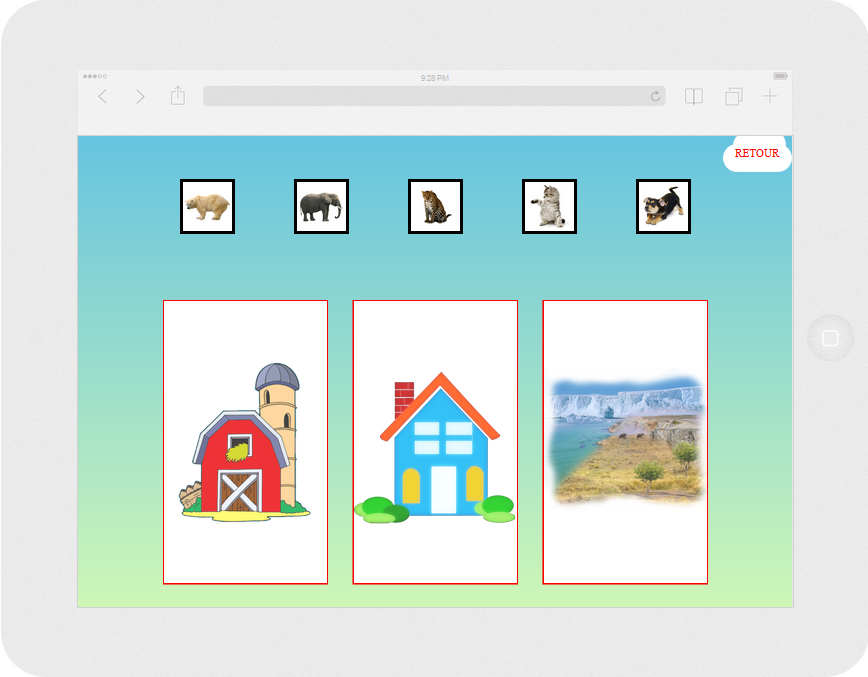
\includegraphics[width=1.0\textwidth]{zone7}
\vspace{0.5cm}\\

\newpage
\section{\'Evolutions}

I'm perfect, so does my game !

\newpage
\section{Outils n\'ecessaires au d\'eveloppement}

\hspace*{0.6cm}Le jeu a \'et\'e enti\`erement cod\'e et r\'ealis\'e en HTML5, CSS et JAVASCRIPT via la librairie JQUERY. Les fichiers du jeu sont lisibles et interpr\'et\'es par tout les navigateurs existants en 2015.\\
\hspace*{0.6cm}Nous avons aussi utilis\'e LaTeX pour \'etablir nos documents textuelles, les diff\'erents navigateurs internet pour \'essayer le jeu ainsi que Photoshop pour la modification des images.\\
Pour partager le code efficacement, nous avons utilis\'e GIT.

\end{document}